\documentclass{article}
\usepackage{amssymb}
\usepackage{amsmath}
\usepackage{mathtools}
\usepackage{centernot}
\usepackage{algpseudocode}
\usepackage{graphicx}
\usepackage[margin=1in]{geometry}
\setlength{\parindent}{0in}

\begin{document}

\title{EE360C: Homework 4}
\author{Joshua Dong (jid295)}
\date{\today}
\maketitle

\section*{1. Coin Changing}
\subsection*{a) greedy}
\begin{algorithmic}
\State {$Quarters := \lfloor n / 25 \rfloor$}
\State {$rem := n \mod 25$}
\State {$Dimes := \lfloor rem / 10 \rfloor$}
\State {$rem := rem \mod 10$}
\State {$Nickels := \lfloor rem / 5 \rfloor$}
\State {$Pennies := rem \mod 5$}
\end{algorithmic}
We show by direct proof that for all integers $n$, the greedy algorithm
preferring the highest denomination provides the optimal solution.
\\\\
A collection of $n/25$ quarters is the most optimal way to make change for any
multiple of 25. This is because a quarter is the maximum denomination, and
thus provides the minimum number of coins used for any multiple of 25. Then
the greedy algorithm provides the most optimal solution for $n$ when
$n \mod 25 = 0$ (trivial case with $n = 0$).

Suppose
$n \mod 25 \in \{0, 1, 2, 3, 4\}$.
Pennies must be used for the remainder no matter what combination is used,
since
$n \mod 25 \in \{0, 1, 2, 3, 4\}$
implies
$n \mod 10 \in \{0, 1, 2, 3, 4\}$
and
$n \mod 5 \in \{0, 1, 2, 3, 4\}$.
Then the optimal result must be the same as $n - (n \mod 25)$. Then the greedy
algorithm provides the most optimal solution for $n$ when
$n \mod 25 \in \{0, 1, 2, 3, 4\}$, since it will first make quarters then
be forced to make pennies. 

Likewise, suppose
$n \mod 25 \in \{5, 6, 7, 8, 9\}$.
0, 1, 2, 3, or 4 pennies must be used, respectively since
$n \mod 25 \in \{5, 6, 7, 8, 9\}$
implies
$n \mod 5 \in \{0, 1, 2, 3, 4\}$.
Ten is a multiple of 5 and it would be more efficient to use a nickel than
5 pennies, so we do not consider the remainders of 10. After reducing the
penny remainder, we have a problem of $n \mod 25 = 5$. Then the greedy
algorithm would make the correct change since it would make as many
quarters as possible, then a nickel, then the pennies.
\\\\
The case for $n \mod 25 \in \{10, 11, 12, 13, 14\}$ is similar, but with a
dime.
\\\\
The case for $n \mod 25 \in \{15, 16, 17, 18, 19\}$ is similar, but with a
dime and a nickel (since the optimal way to make change for 40 is with a
quarter, a dime, and a nickel.
\\\\
The case for $n \mod 25 \in \{20, 21, 22, 23, 24\}$ is similar, but with two
dimes (since the optimal way to make change for 45 is with a quarter and two
dimes).

\subsection*{b) Counterexample}
Suppose our denominations are $\{1, 5, 7\}$. If $n = 10$, then our greedy
algorithm fails with $7, 1, 1, 1$ instead of $5, 5$.


\section*{2. Intervals}
An example algorithm to find the minimal tiling cover is one that iterates
brute-force through all combinations of X's ($2^n$ distinct subsets) in order
of subset size, then returns the first result that is a tiling cover. This
must be correct since we only return results that are tiling covers, and
always return a tiling cover of smallest size.
\\\\
An example of a greedy algorithm to compute this answer would be an algorithm
that took the leftmost interval (smallest $X_L$) and took the intersecting
interval with the greatest $X_R$ as the next interval. The algorithm would
continue selecting the next interval by selecting the interval with the
greatest $X_R$ value that intersected with the current rightmost interval
until it reached the greatest $X_R$ value.
\\\\
This algorithm is correct since at any point in the algorithm, a tiling cover
is selected for the span from $X_L$ to $X_R$. Any tiling returned by the
greedy algorithm is also optimal since it is optimal at every step, that is,
at every step the algorithm produces a minimal tiling cover of its endpoints.
\\\\
Note that ties in the selection of the first interval are determined by the
best corresponding $X_R$ value.

\section*{3. Greedy Algorithm}
\subsection*{a) minimum stations}
Let $error$ be 0 or 1, depending on if base station coverage is closed or open
in its coverage. $error$ will also be 1 if the line segment has any open
endpoints.
Divide the road length by 8, add $error$, and distribute the base stations
evenly.

\subsection*{b) proof}
Suppose our algorithm requires $n$ stations. If we could accomplish the task
with less than $n$ base stations, then the optimal number of base stations
must be $n - 1$ or less. We make two cases for open and closed set coverage.
\\\\
For the first case, suppose base station coverage is an open set. With $n - 1$
base stations, the separation of base stations is exactly 8. Then there are
a finite number of points not covered by the stations, namely the points at
the midpoint between any two adjacent base stations. If a resident lives at
this point, then they are not covered. Then $n - 1$ or less base stations
cannot cover the line segment. With $n$ base stations, the distance between
stations is less than 8. Then every point on the line segment in in the open
ball of radius 4 of a base station. We use similar arguments to argue set
coverage when there exist one or more open endpoints.
\\\\
For the second case, base station coverage is a closed set. With $n - 1$ base
stations, the distance between any two base stations is greater than 8. Then
the midpoint between any two adjacent base stations is not in any radius 4
ball of a base station. Then $n - 1$ or less base stations cannot cover the
line segment because a ball of radius $(n - 1) * 4$ can contain all base
stations, but is smaller than the line segment. With $n$ base stations, the
distance between stations is exactly 8 and we can have a cover of the line
segment. Then $n$ is the smallest possible number of base stations.
\\\\
Then in all cases, the greedy algorithm produces a cover of the line segment
that is also minimal.

\newpage
\section*{4. Single Source Shortest Paths}
\subsection*{a) Dijkstra Time}
The time is bounded by $O(n)$, but varies greatly depending on $u$, $v$, and
the graph.

\subsection*{b) Faster than Dijkstra}
If $v$ is in the subtree of $u$, then return the path from $u$ to $v$, since
there is only one such path. Otherwise, compute the best path from $u$ to the
root (can use Dijkstra's algorithm here). Then add the path from the root to
$v$ to the patch from $u$ to the root. While this can be much faster, the time
complexity is similar in worst-case behaviour but much better on average.

\section*{5. Shortest Paths}
No. Otherwise a greedy algorithm would work for generating minimum spanning
trees. See the image for a counterexample.

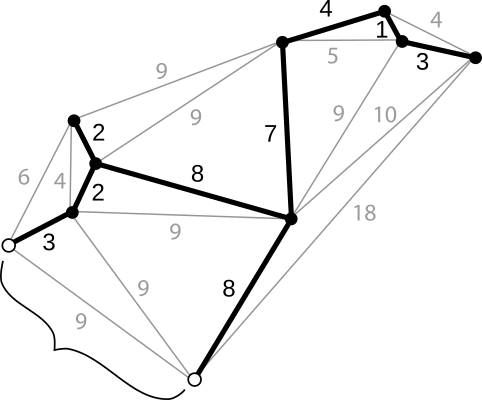
\includegraphics[width=240px]{graphs/mst.png}

\section*{6. Minimum Spanning Trees}
Add all edges to the minimum spanning tree. Take all $2^9$ combinations of
edges removed from this tree and test if they are connected (this is still
$O(n)$ when done with proper data structures, especially considering only
updated verticies need to be checked). Then find the minimum of these
combinations, a $O(1)$ operation as this does not become more difficult with
an increasing number of nodes.
\\\\
This algorithm is correct since it returns a spanning tree after checking
updated verticies for connectivity. This algorithm also returns the
minimum spanning tree since it sorts the constant number of results and
returns the smallest of the results.

\section*{7. Huffman Coding}
Let $C$ be a prefix code encoding in a binary tree representing that is not
full. Then there exists a node $x$ with only one child. Let $C'$ be a tree
identical to $C$ but with the subtree of $x$ removed, the prefixes pushed into
$x$. Since the lengths of the prefixes in the subtree of $x$ are longer than
the prefix of $x$, the average must be smaller now
($\sum_{ i = A_i }^n { p(A_i) } = p(x)$ where $A_i$ is the $i$th prefix
under $x$ and $n$ is the number of prefixes under $x$). Then a binary tree
that is not full cannot correspond to an optimal prefix code.

\end{document}both 
